\documentclass[twoside, a4paper, 11pt]{article}
\usepackage[utf8x]{inputenc}
\usepackage[T1]{fontenc}
\usepackage{times}
\usepackage{anysize}
\usepackage{fancyhdr}
\usepackage{pdfpages}
\usepackage{tabularx}

\marginsize{3cm}{2cm}{2cm}{2cm}

% Indicador completo en lugar de página
\fancyfoot[C]{{\ttfamily RTF PR:2.0 \quad \thepage}}
\renewcommand*{\headrulewidth}{0pt}
\pagestyle{fancy}

% Comando para indicar los problemas
\newcommand{\problema}[2]{\begin{description} \item[Exposición] #1 \item[Resolución] #2 \end{description}}

\begin{document}
	% Título
	\begin{center}
		\scshape \large Acta de la Revisión Técnica Formal \textit{Plan de proyecto} - Grupo Diedral \vspace{.5cm}
	\end{center}

	Reunidos Juan Andrés Claramunt Pérez y Rubén Rafael Rubio Cuéllar como representantes de la parte revisada, el Grupo Diedral; y Enrique Ballesteros Horcajo, Jaime Dan Porras Rhee e Ignacio Iker Prado Rujas  por la parte revisora, el equipo PKT; en el laboratorio 10 de la Facultad de Informática de la Universidad Complutense de Madrid a viernes 8 de marzo de 2013 a las 13:00, se procede a la Revisión Técnica Formal del documento ``Plan de proyecto'' con número de registro PR:2.0 perteneciente al Grupo Diedral.\\

	El equipo revisor presenta un documento, anexo a al presente, con sus conclusiones previas. Se tratan los siguientes temas por orden de aparición:

	\begin{enumerate}
		\renewcommand*{\theenumi}{P\arabic{enumi}}
		
		\item \problema{Los apartados ámbito del proyecto y funciones principales no están claramente\break diferenciados.}{El Grupo Diedral reconoce la semejanza y se compromete a su edición.}
		\item \problema{El equipo revisor sugiere que en el apartado restricciones y técnicas de gestión se trate el tema de seguridad frente a terrorismo.}{Se toma la sugerencia en consideración.}
		\item \problema{En el apartado 2.1 datos históricos se hace referencia a gestión de riesgos cuando debería tratar de estimaciones.}{El Grupo Diedral reconoce el error y se compromete a su correción.}
		\item \problema{En la estimación de puntos de función, al campo dirección se le asignan 6 DET pero no se especifican.}{Se rechaza la sugerencia puesto que están especificados en las SRS en las que se basan.}
		\item \problema{En algunas tablas de estimación de puntos de función se mencionan FTR cuando deberían ser RET.}{El equipo de desarrollo admite el error y se compromete a su reparación.}
		\item \problema{El equipo revisor sugiere indicar explicitamente el caso en que alguno de los campos de las tablas de puntos de función quedasee vacío.}{No se llega a ninguna conclusión.}
		\item \problema{En algunas tablas falta el campo de complejidad.}{Se admite el error y se acuerda su corrección.}
		\item \problema{Falta puntos de función ajustados.}{La parte revisada admite que se han calculado y serán incluidos.}
		\item \problema{El equipo revisor sugiere la inclusión de una leyenda con la identificación de las iniciales usadas en la tabla de riesgos}{Se admite la sugerencia y será añadida la correspondiente leyenda.}
		\item \problema{En cada tabla de riesgo hay un apartado de detonantes y acción de contingencias sin embargo solo se trata la acción de contingencia.}{Se admite el error y queda pendiente de corregir.} %?
		\item \problema{Se sugieren cambios en el formato de las tablas.}{Se toman en consideración.}
		\item \problema{Falta tabla de recursos del proyecto.}{Se admite y será añadida.}
		\item \problema{Se sugiere describir los tipos de licencia LPPL y GPL.}{Se considera añadir un enlace a la descripción completa de dichas licencias.}
		\end{enumerate}

	\vspace*{1cm}

	Quedan de acuerdo sobre la fidelidad de estos puntos a los hechos acaecidos en la fecha y lugar\break anteriormente reseñados, el Grupo Diedral y PKT, por vía de sus representantes plenipotenciarios.\\

	% Espacio (casi de medida 0) para las firmas
	\begin{tabularx}{.9\linewidth}{X  >{\raggedleft}X}
		El Grupo Diedral & PKT
	\end{tabularx}

	% Indica que viene el anexo
	\vfill{}
	{\itshape A continuación se incluye el anexo elaborado por el equipo revisor:}

	% Incluye el anexo del otro grupo
	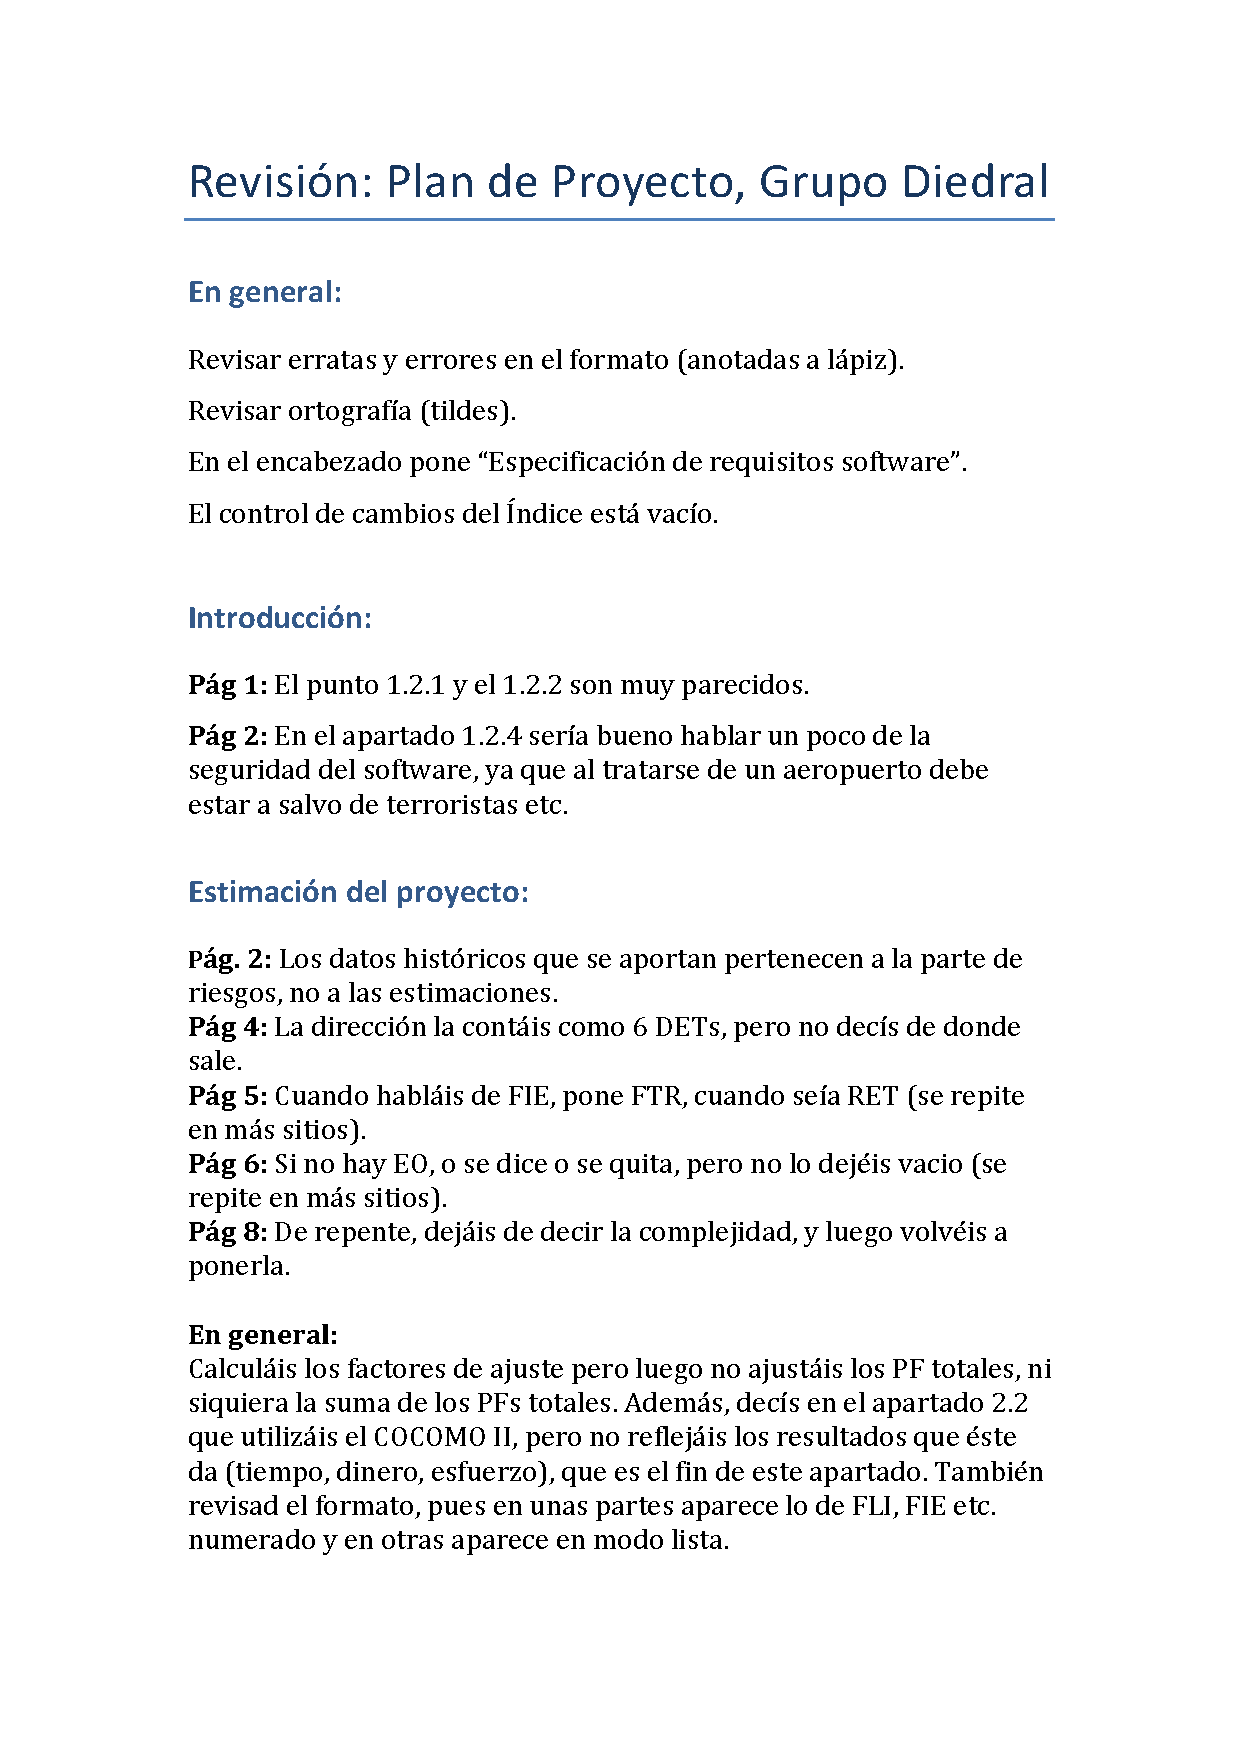
\includepdf[pages=1-2, pagecommand={}]{revplan_anexo.pdf}
\end{document}
